\documentclass{beamer}
\usepackage{amsmath}
\usepackage{xcolor}
\usepackage{multimedia}
\usepackage{bbm}
\usepackage{dsfont}
\usepackage{wrapfig}
\usetheme{Copenhagen}
\definecolor{purple}{rgb}{0.3,0,0.4}
\definecolor{aqua}{rgb}{0,0.85,0.8}
\definecolor{grey}{rgb}{60,60,60}
\setbeamercolor*{palette primary}{use=structure, fg=white, bg=purple}
\setbeamercolor*{background canvas}{bg=purple!5}
\setbeamercolor*{block title example}{use=structure,fg=white,bg=purple}
\setbeamercolor*{block body example}{fg=black,use=block title,bg=purple!20}
\setbeamercolor*{block title}{use=example text,fg=white,bg=aqua!60!black}
\setbeamercolor*{block body}{fg=black,use=block title example,bg=aqua!10}

\usepackage{graphicx}
\usepackage{tikz-cd}

\newcommand{\Gal}{\mathrm{Gal}}
\newcommand{\Cl}{\mathrm{Cl}}
\newcommand{\BSD}{\mathrm{BSD}}
\newcommand{\tors}{\mathrm{tors}}
\newcommand{\Reg}{\mathrm{Reg}}
\newcommand{\rk}{\mathrm{rk}}
\newcommand{\trivial}{\mathbbm{1}}
\newcommand{\Ind}{\mathrm{Ind}}
\newcommand{\Rep}{\mathrm{Rep}}
\newcommand{\Tr}{\mathrm{Tr}}
\newcommand{\Stab}{\mathrm{Stab}} 
\newcommand{\Res}{\mathrm{Res}}
\newcommand{\GL}{\mathrm{GL}}
\newcommand{\ord}{\mathrm{ord}}


\newcommand{\CC}{\mathbb{C}}
\newcommand{\FF}{\mathbb{F}}
\newcommand{\NN}{\mathbb{N}}
\newcommand{\PP}{\mathfrak{P}}
\newcommand{\QQ}{\mathbb{Q}}
\newcommand{\RR}{\mathbb{R}}
\newcommand{\ZZ}{\mathbb{Z}}
\newcommand{\GG}{\mathbb{G}}
\newcommand{\adele}{\mathbb{A}}
\newcommand{\pp}{\mathfrak{p}}
\newcommand{\qq}{\mathfrak{q}}
\newcommand{\rr}{\mathfrak{r}}
\newcommand{\af}{\mathfrak{a}}
\newcommand{\fg}{\mathfrak{g}}
\newcommand{\bQ}{\mathbb{Q}}
\newcommand{\bC}{\mathbb{C}}
\newcommand{\bZ}{\mathbb{Z}}
\newcommand{\fP}{\mathfrak{P}}
\newcommand{\fp}{\mathfrak{p}}
\newcommand{\fw}{\mathfrak{w}}
\newcommand{\fN}{\mathfrak{N}}
\newcommand{\fq}{\mathfrak{q}}
\newcommand{\cO}{\mathcal{O}}
\newcommand{\repnorm}[1]{\fN_{\bQ(#1) / \bQ}(#1)}

%Sha:
\usepackage[OT2,T1]{fontenc}
\DeclareSymbolFont{cyrletters}{OT2}{wncyr}{m}{n}
\DeclareMathSymbol{\Sha}{\mathalpha}{cyrletters}{"58}
%end of Sha

\theoremstyle{plain}
\newtheorem{thm}{Theorem}[section]
\newtheorem{rem}[thm]{Remark}
\newtheorem{proposition}[thm]{Proposition}
\newtheorem{conjecture}[thm]{Conjecture}
\newtheorem{deflem}[thm]{Definition/Lemma}
\newtheorem{question}[thm]{Question}


\graphicspath{ }


\title[Artin Formalism]{A Study of the Arithmetic Consequences of Artin Formalism for
Predicting Positive Rank}
\author{Edwina Aylward, Albert Lopez Bruch}
%\institute{LSGNT}
\date{21 May, 2024}

\begin{document}

\frame{\titlepage}

\begin{frame}{Table of contents}
    +notation
\end{frame}

\begin{frame}
    \frametitle{Elliptic Curves}
    Let $K$ be a field. Any elliptic curve over $K$ can be written as the locus on $\mathbb{P}^2$ of a \textbf{Weierstrass equation}
    \begin{equation}
        E:y^2+a_1xy+a_3y=x^3+a_2x^2+a_4x+a_6,\quad a_i\in K
    \end{equation}
    together with $[0:1:0]$ at infinity, and it has an associated discriminant $\Delta\neq0$. 
    \\~\\
    When $\Delta=0$, the equation above defines a singular cubic curve, and two behaviours can occur.
    
    \centering
    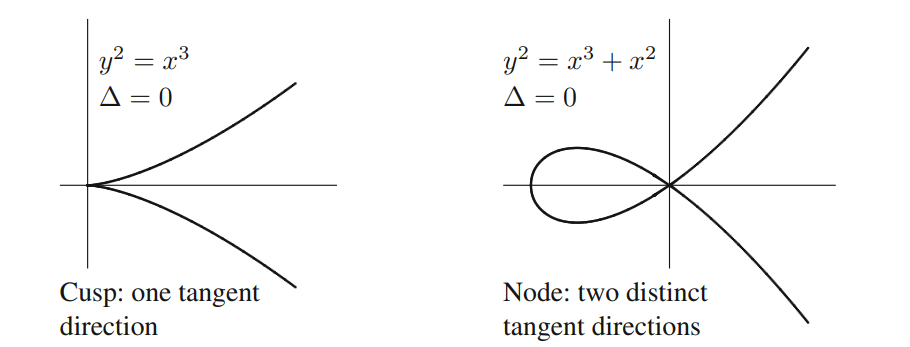
\includegraphics[scale=0.4]{Singular_cubic.png}
\end{frame}

\begin{frame}
    \frametitle{The Mordell--Weil Group}
    Let $K$ be a field and let $E$ be an elliptic curve over $K$. The set of $K$-points of $E$ form an abelian group $E(K)$. 
    \begin{theorem}[Mordell--Weil]
        Let $K$ be a number field and let $E$ be an elliptic curve over $K$. Then $E(K)$ is a finitely generated abelian group.
    \end{theorem}
    Consequently, $E(K)\cong E(K)_{tors}\times\ZZ^r$, where $r$ is denoted the \textbf{rank} of the elliptic curve.

    %\centering
    %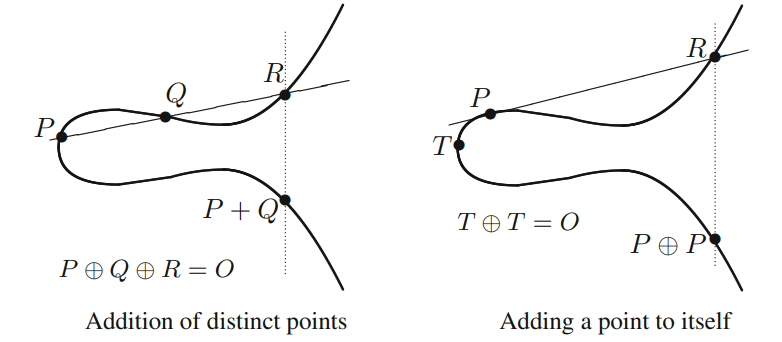
\includegraphics[scale=0.4]{MW_group.png}
\end{frame}

\begin{frame}
    \frametitle{Reduction of an Elliptic Curve}
    Suppose $K$ is a local field with $\mathrm{char}(K)=0$, discrete valuation $\nu$, valuation ring $R$ and max ideal $\mathfrak{m}$ and residue field $\kappa=R/\mathfrak{m}$.
    \begin{definition}
        A Weierstrass equation for $E/K$ is \textbf{minimal} if $a_i\in R$ and $\nu(\Delta)$ is minimal among all such equations.
    \end{definition}
    When the Weierstrass equation is minimal, we have an associated curve $\tilde{E}$ over $\kappa$ (which could be singular!) and a reduction map 
    $$\widetilde{(\cdot)}:E(K)\longrightarrow \tilde{E}(\kappa)$$
    by reducing the coordinates modulo $\mathfrak{m}$.
\end{frame}

\begin{frame}
    \frametitle{Reduction Types}
    The reduction type of $E$ over $K$ describes the behaviour of $\tilde{E}/\kappa$.
    \begin{definition}
        We say that
        \begin{enumerate}%[label={(\alph*)}]
            \item $E/K$ has \textbf{good} reduction if $\tilde{E}$ is non-singular (i.e. $\nu(\Delta)=0$).
            \item $E/K$ has \textbf{multiplicative} reduction if $\tilde{E}$ has a node.
            \item $E/K$ has \textbf{additive} reduction if $\tilde{E}$ has a cusp.
        \end{enumerate}
        If $E/K$ has multiplicative reduction, then we say that the reduction is \textbf{split} if the slopes of the tangent lines at the node lie in $\kappa$, and \textbf{non-split} otherwise.
    \end{definition}

\end{frame}

\iffalse
\begin{frame}
    \frametitle{Reduction Types}
    The reduction type of $E$ over $K$ describes the behaviour of $\tilde{E}/\kappa$.
    \begin{definition}
        We say that
        \begin{enumerate}%[label={(\alph*)}]
            \item $E/K$ has \textbf{good} reduction if $\tilde{E}$ is non-singular (i.e. $\nu(\Delta)=0$).
            \item $E/K$ has \textbf{multiplicative} reduction if $\tilde{E}$ has a node.
            \item $E/K$ has \textbf{additive} reduction if $\tilde{E}$ has a cusp.
        \end{enumerate}
    \end{definition}
    \begin{proposition}
        Let $E$ be an elliptic curve over a local field $K$ of characteristic $0$. 
        \begin{enumerate}
            \item If $F/K$ unramified, the reduction of $E/K$ equals that of $E/F$.
            \item If $F/K$ is finite and $E/K$ is good or multiplicative, then $E/F$ has the same reduction.
            % \item If $E$ has non-split multiplicative reduction over $K$ and $F/K$ is a finite extension with even residual degree, then $E$ has split multiplicative reduction over $F$. 
            \item There exists a finite extension $F/K$ such that $E/F$ is either good or multiplicative.
        \end{enumerate}
    \end{proposition}
\end{frame}


\begin{frame}
    \frametitle{Multiplicative Reduction}
    \begin{definition}
        Suppose that $E/K$ has multiplicative reduction. Then we say that the reduction is \textbf{split} if the slopes of the tangent lines at the node lie in $\kappa$, and \textbf{non-split} otherwise.
    \end{definition}
    \begin{proposition}
        Let $E$ be an elliptic curve over a local field $K$ of characteristic $0$. 
        \begin{enumerate}
            \item If $F/K$ is finite and $E/K$ is split multiplicative, then $E/F$ has the same reduction.
            \item If $F/K$ has even residual degree and $E/K$ is non-split, then $E/F$ is split.
            \item There exists a finite extension $F/K$ such that $E/F$ is either good or split multiplicative.
        \end{enumerate}
    \end{proposition}   
\end{frame}
\fi



\begin{frame}
    \frametitle{L-function of an Elliptic Curve}
    Let $K$ be a number field and let $E$ be an elliptic curve over $K$.
    \begin{definition}
        If $\pp$ is a finite place of $K$, let $q_\pp=|\kappa_\pp|$ and $a_\pp=1+q_\pp-|\tilde{E}(\kappa_\pp)|$. The local polynomial of $E$ at $\pp$ is defined as
        \[
            P_\pp(E,T)=
            \begin{cases}
                1-a_\pp T+q_\pp T^2 &\text{ if $E/K_\pp$ good,}\\
                1-T &\text{ if $E/K_\pp$ split multiplicative,}\\
                1+T &\text{ if $E/K_\pp$ nonsplit multiplicative,}\\    
                1 &\text{ if $E/K_\pp$ additive.}
            \end{cases}
        \]
    Then the L-function attached to $E$ is 
    $$L(E/K,s)=\prod_{\pp\text{ prime}}\frac{1}{P_\pp(E,N(\pp)^{-s})}.$$
    \end{definition}
    We remark that $L(E/K,s)$ is holomorphic in some half plane.
\end{frame}

\begin{frame}
    \frametitle{Artin Representations}
    \begin{definition}
        Let $K$ be a field. An Artin representation $\rho$ is a complex finite dimensional vector space $V$ together with a homomorphism $\rho:G_K\to\GL(V)$ such that $\Gal(\bar{K}/F)\subseteq\ker\rho$ for some finite Galois extension $F/K$.
    \end{definition}
    Effectively, Artin representations of $K$ are finite dimensional reps of $\Gal(F/K)$ for some finite extension $F/K$.
    \begin{rem}
        Let $L/K$ be a finite extension of number fields and $\rho$ an Artin rep of $L$ factoring through $\Gal(F/L)$. 
        Then $\Ind_{G_L}^{G_K}\rho$ is an Artin rep factoring through $\Gal(F/K)$, which is equivalent to 
        $$\Ind_{\Gal(F/L)}^{\Gal(F/K)}\rho.$$
    \end{rem}
\end{frame}

\begin{frame}
    \frametitle{Artin Twists and Artin Formalism}
    Given an elliptic curve $E$ and an Artin representation $\rho$ over a number field $K$, we can construct an L-function $L(E/K,\rho,s)$.

    \begin{theorem}[Artin Formalism]
        Let $E$ be an elliptic curve over a number field $K$. 
        \begin{enumerate}
            \item For Artin representations $\rho_1,\rho_2$ over $K$,
            $$L(E/K,\rho_1\oplus\rho_2,s)=L(E/K,\rho_1,s)L(E/K,\rho_2,s).$$
            \item If $L/K$ is a finite extension and $\rho$ is an Artin representation over $L$,
            $$L(E/L,\rho,s)=L(E/K,\Ind_{G_L}^{G_K}\rho,s).$$
            \item If $L/K$ as above and 
            $\Ind_{L/K}\mathds{1}\cong\bigoplus_i\rho_i,$
            then 
            $$L(E/L,s)=\prod_i L(E/K,\rho_i,s).$$
        \end{enumerate}        
    \end{theorem}
\end{frame}

\begin{frame}
    \frametitle{An $S_3$ Example}
    Let $E$ be an elliptic curve over $\QQ$. Consider $L=\QQ(\sqrt[3]{2},\zeta_3)$ and note that $\Gal(L/\QQ)=S_3$. 
    \begin{table}[]
        \begin{tabular}{|c|c c c|}
            \hline
                        & $e$ & $(1,2)$ & $(1,2,3)$ \\ \hline
            $\mathds{1}$  & 1   & 1       & 1         \\ 
            $\varepsilon$ & 1   & -1      & 1         \\ 
            $\rho$        & 2   & 0       & -1        \\ \hline
        \end{tabular}
        \caption[short]{Character table for $S_3$}
    \end{table}
    By viewing all Artin reps as reps of $S_3$, Artin formalism gives
    \begin{itemize}
        \item $L(E/\QQ(\sqrt[3]{2},\zeta_3))=L(E,\mathds{1},s)L(E,\varepsilon,s)L(E,\rho,s)^2$
        \item $L(E/\QQ(\sqrt[3]{2}))=L(E,\mathds{1},s)L(E,\rho,s)$
        \item $L(E/\QQ(\zeta_3))=L(E,\mathds{1},s)L(E,\varepsilon,s)$.
    \end{itemize}
    Therefore,
    $$L(E/\QQ(\sqrt[3]{2},\zeta_3),s)L(E/\QQ,s)^2=L(E/\QQ(\zeta_3),s)L(E/\QQ(\sqrt[3]{2}),s)^2$$    
\end{frame}

\begin{frame}
    \frametitle{Birch and Swinnerton-Dyer Conjecture}
    \begin{conjecture}[Birch--Swinnerton-Dyer]
        Let $E$ be an elliptic curve defined over a number field $F$. Then 
        \begin{enumerate}%[label={\bfseries  BSD\arabic*.}]
            \item The rank of the Mordell-Weil group of $E$ over $F$ equals the order of vanishing of the $L$-function; that is,
            $$\ord_{s=1}L(E/F,s)=\rk E/F = r.$$
            \item The group $\Sha_{E / F}$ has finite order and the leading term of the Taylor series at $s=1$ of the $L$-function is
            \begin{equation*}\label{BSD_2}
                \lim_{s\to1}\frac{L(E/F,s)}{(s-1)^r}\cdot\frac{\sqrt{|\Delta_F|}}{\Omega_+(E)^{r_1+r_2}|\Omega_-(E)|^{r_2}}=\frac{\Reg_{E/F}|\Sha_{E/F}|C_{E/F}}{|E(F)_{\tors}|^2}.
            \end{equation*}
        \end{enumerate}
    \end{conjecture}
    

\end{frame}

\begin{frame}
    \frametitle{Birch and Swinnerton-Dyer for Artin Twists}
    %\begin{definition}
        %For an elliptic curve $E$ over a number field $K$, let
        %$$\BSD(E/K):=\frac{\Reg_{E/K}|\Sha_{E/K}|C_{E/K}}{|E(K)_{\tors}|^2}.$$
    %\end{definition}
    \begin{conjecture}[BSD1 for Artin Twists]
        Let $E/\QQ$ be an elliptic curve, $\rho$ an Artin representation and $F/\QQ$ a Galois extension $\QQ$ such that $\rho$ factors through $Gal(F/\QQ)$. Then
        $$\ord_{s=1}L(E,\rho,s)=\langle\rho,E(F)_\CC\rangle,$$
        where $E(F)_\CC=E(F)\otimes_\ZZ \CC$ is viewed as a $\Gal(F/\QQ)$ representation and $\langle\cdot,\cdot\rangle$ is the usual inner product of characters.
    \end{conjecture}
    \textbf{Problem:} Can we formulate a BSD2 analogue for Artin Twists?
\end{frame}

\begin{frame}
    \frametitle{Arithmetic and Analytic Information}
    The BSD conjecture gives a way to obtain arithmetic information from analytic and viceversa.
    \begin{example}
        Isogenous elliptic curves have the same L-function. Hence, BSD predicts that their rank and leading terms of the L-functions at $s=1$ are equal. The former is elementary, but the later is a deep result by Cassels.
    \end{example}
    \begin{example}
        Let $\rho$ be an Artin representation over $\QQ$ that factors through $\Gal(F/\QQ)$. If $\rho^\mathfrak{g}$ is the representation such that $\Tr\circ \rho^\mathfrak{g}=\mathfrak{g}(\Tr\circ\rho)$ for some $\mathfrak{g}\in\Gal(\QQ(\rho)/\QQ)$, then $$\langle\rho,E(F)_\CC\rangle=\langle\rho^\mathfrak{g},E(F)_\CC\rangle.$$
        Thus, BSD then predicts $\ord_{s=1}L(E,\rho,s)=\ord_{s=1}L(E,\rho^\mathfrak{g},s)$.
    \end{example}
\end{frame}

\begin{frame}
    \frametitle{Arithmetic and Analytic Information}
    \begin{example}
        From the $S_3$ example, BSD1 predicts that $$\rk E/\QQ(\sqrt[3]{2},\zeta_3)+2\rk E/\QQ=\rk E/\QQ(\zeta_3)+2\rk E/\QQ(\sqrt[3]{2}).$$
        Let $V=E(\QQ(\sqrt[3]{2},\zeta_3))\otimes_\ZZ \CC$, which is naturally a $\CC S_3$-module. Then
        \begin{itemize}
            \item $\rk E/\QQ=\dim V^{S_3}= \langle V,\mathds{1}\rangle$,
            \item $\rk E/\QQ(\zeta_3)=\dim V^{C_3}=\langle V,\mathds{1}\oplus\varepsilon\rangle$,
            \item $\rk E/\QQ(\sqrt[3]{2})=\dim V^{C_2}=\langle V,\mathds{1}\oplus\rho\rangle$,
            \item $\rk E/\QQ(\sqrt[3]{2},\zeta_3)=\dim V=\langle V,\mathds{1}\oplus\varepsilon\oplus\rho^2\rangle$.
        \end{itemize}
    \end{example}

\end{frame}

\begin{frame}
    \frametitle{BSD term}
    We discard some of the BSD terms for $E / K$
    and define  

    \begin{definition}
        $$\BSD(E / K) = \frac{\Reg_{E / K}|\Sha_{E / K}| C_{E / K}}{|E(K)_{\tors}|^2 }$$
    \end{definition}
    \pause

    Suppose $\rk E / K = 0$. Then $\Reg_{E / K} = 1$. Assuming finiteness of $\Sha_{E / K}$, Cassels proved that $|\Sha_{E / K}|$ is a square. \pause Thus one has
    $$ \BSD(E / K) \equiv C_{E / K} \mod (\QQ^{\times})^2. $$
\end{frame}
%\end{section}

\begin{frame}
    \frametitle{Artin formalism for BSD}
    Consider $E / \QQ$, and $F / \QQ$ with $G = \Gal(F / \QQ)$.  \pause
    As in the $L$-function case, we would like to be able to break up $\BSD(E / F)$ according to representations of $G$. \pause
    
    \begin{conjecture}[BSD-term conjecture]
        For each representation $\rho$ of $G$, there exists an invariant $\BSD(E, \rho) \in \CC^{\times}$ such that:\pause
        \begin{enumerate}
            \item$\BSD(E / F^H) = \BSD(E, \Ind_H^G \trivial)$ for $H \leq G$, \pause
            \item $\BSD(E, \rho \oplus \tau) = \BSD(E, \rho)\BSD(E , \tau)$, where $\tau \in \Rep(G)$.\pause
        \end{enumerate}
    \end{conjecture}

    Therefore, if $\Ind_H^G \trivial \simeq \trivial \oplus \bigoplus_i \rho_i$, one has
    $$ \BSD(E / F^H) = \BSD(E / \QQ)\prod_i \BSD(E, \rho_i). $$ 
\end{frame}

\begin{frame}
    \frametitle{Artin formalism for BSD}
This conjecture is studied in \cite{DEW1}. They show it is true assuming some well-known conjectures. \pause They also conjecture (and justify) an additional useful property: 

\begin{conjecture}[BSD-term conjecture]
    For each representation $\rho$ of $G$, there exists an invariant $\BSD(E, \rho) \in \CC^{\times}$, satisfying the previous properties, \pause such that if $\langle \rho, E(F)_{\CC} \rangle = 0$, then
    \begin{enumerate}\setcounter{enumi}{2}
        \item Galois equivariance: $\BSD(E, \rho) \in \QQ(\rho)^{\times}$ and $$\BSD(E, \rho^{\mathfrak{g}}) = \BSD(E, \rho)^{\mathfrak{g}} \text{ for } \mathfrak{g} \in \Gal(\bQ(\rho) / \bQ).$$ 
    \end{enumerate}

\end{conjecture}
\end{frame}

%\begin{frame}
%    \frametitle{Artin formalism for BSD}
%    \begin{conjecture}
%        For each representation $\rho$ of $G$, there exists an invariant $\BSD(E, \rho) \in \CC^{\times}$ (as before)  such that if $\langle \rho, E(F)_{\CC} \rangle = 0$, then
%        \begin{enumerate}\setcounter{enumi}{2}
%            \item Galois equivariance: $\BSD(E, \rho) \in \QQ(\rho)^{\times}$ and $$\BSD(E, \rho^{\mathfrak{g}}) = \BSD(E, \rho)^{\mathfrak{g}} \text{ for } \mathfrak{g} \in \Gal(\bQ(\rho) / \bQ).$$ 
%        \end{enumerate}
    
%    \end{conjecture}
%    \pause
%    Here 
%    \begin{itemize}
%        \item $E(F)_{\bC} = E(F) \otimes_{\bZ} \bC$ is viewed as a $G$-representation, \pause
%        \item $\langle -, - \rangle$ is the usual inner product of characters of $G$, \pause
%       \item $\bQ(\rho)$ is an abelian extension of $\bQ$ obtained by adding $\{ \Tr \rho(\fg) \colon \fg \in G \}$ to $\bQ$, \pause
%        \item $\rho^{\fg}$ is the representation of $G$ with character $\Tr \rho^{\fg} = \fg \circ \Tr \rho $.
%    \end{itemize}

%\end{frame}

\begin{frame}
    \frametitle{Norm Relations Test}
    Again, consider $E/ \bQ$, $F / \bQ$ and $G = \Gal(F / \bQ)$. \pause Take a representation $\rho$ of $G$, and assume $\langle \rho, E(F)_{\bC} \rangle = 0$. Then 
    $$ \repnorm{\rho} := \bigoplus_{\fg \in \Gal(\bQ(\rho) / \bQ)} \rho^{\fg}$$
    has rational character. \pause 
    The BSD-term conjecture implies that
    $$\BSD(E, \bigoplus_{\fg \in \Gal(\bQ(\rho) / \bQ)} \rho^{\fg}) = \prod_{\fg \in \Gal(\bQ(\rho) / \bQ)} \BSD(E, \rho)^{\fg}$$\pause
    is the norm of an element from $\bQ(\rho)^{\times}$. 
\end{frame}

\begin{frame}
    \frametitle{Norm relations test}
    There exists some $m \geq 1$ such that $$\bigg(\bigoplus_{\fg \in \Gal(\bQ(\rho) / \bQ)} \rho^{\fg}\bigg)^{\oplus m}$$
    can be written in terms of permutation representations, i.e. \pause
    $$  \bigg(\bigoplus_{\fg \in \Gal(\bQ(\rho) / \bQ)} \rho^{\fg}\bigg)^{\oplus m} \simeq \bigoplus_{i} \Ind_{H_i}^G \trivial \ominus \bigoplus_{j} \Ind_{H_j'}^G \trivial$$
    for some $H_i$, $H_j' \leq G$. 
\end{frame}

\begin{frame}
    \frametitle{Norm Relations Test}
    $$\bigg(\bigoplus_{\fg \in \Gal(\bQ(\rho) / \bQ)} \rho^{\fg}\bigg)^{\oplus m} \simeq \bigoplus_{i} \Ind_{H_i}^G \trivial \ominus \bigoplus_{j} \Ind_{H_j'}^G \trivial$$ \pause
    On the level of BSD terms we get
    $$\bigg(\prod_{\fg \in \Gal(\bQ(\rho) / \bQ)} \BSD(E, \rho)^{\fg}\bigg)^m = \frac{\prod_i \BSD(E / F^{H_i})}{\prod_j \BSD(E / F^{H_j'})} ,$$
    \pause so the left hand side is the norm of an element of $\bQ(\rho)$. \pause It is also the norm of an element from any subfield of $\bQ(\rho)$. 
\end{frame}

\begin{frame}
    \frametitle{Norm Relations Test}
    Now assume $\rk E / F = 0$. Then for all $H \leq G$, 
    $$ \BSD(E / F^{H}) \equiv C_{E / F^H} \mod (\bQ)^{\times 2}.$$ \pause
    Squares are norms from quadratic fields. \pause Thus if $\bQ(\sqrt{D}) \subset \bQ(\rho)$, then 
   $$\frac{\prod_i \BSD(E / F^{H_i})}{\prod_j \BSD(E / F^{H_j'})} \in N_{\bQ(\sqrt{D}) / \bQ}(\bQ(\sqrt{D})^{\times})$$ \pause $$\implies 
   \frac{\prod_i C_{E / F^{H_i}}}{\prod_j C_{E / F^{H_j'}}} \in N_{\bQ(\sqrt{D}) / \bQ}(\bQ(\sqrt{D}^{\times})). $$\pause
   \textbf{so if this product isn't a norm...\pause our rank assumption was wrong!}
\end{frame}

\begin{frame}
    \frametitle{Norm Relations Test}
    %We have deduced the following:
    \begin{theorem}[{Norm Relations Test, \cite[Theorem 33]{DEW1}}]\label{thm_positive_rank}
    \small{  Suppose our conjecture for the BSD terms holds. Consider $E/\QQ$, and $F/\QQ$  with $G = \Gal(F / \bQ)$. Let $\rho$ be a representation of $G$, and let $\bQ(\sqrt{D}) \subset \bQ(\rho)$. Suppose we have  
        $$\left(\bigoplus_{\mathfrak{g}\in\Gal(\QQ(\rho)/\QQ)}\rho^{\mathfrak{g}}\right)^{\oplus m}=\bigoplus_i\Ind_{H_i}^G\mathbbm{1}\ominus\bigoplus_j\Ind_{H'_j}^G\mathbbm{1}$$
        for some $m\geq 1$ and $H_i, H_j' \leq G$. If 
        $$\frac{\prod_i C_{E/F^{H_i}}}{\prod_j C_{E/F^{H_j'}}} \not\in
        \begin{cases}
            (\bQ)^{\times 2} & m \text{ even,}\\
            N_{\bQ(\sqrt{D}) / \bQ}(\bQ(\sqrt{D})^{\times}) & m \text{ odd,}
        \end{cases}
        $$
        then $\rk E / F > 0.$ }
    \end{theorem}
\end{frame}

\begin{frame}{Parity conjecture and parity tests}
    A more common method of forcing positive rank for an elliptic curve $E / K$ is by use of the parity conjecture:
    \begin{conjecture}[Parity conjecture]\label{parity}
            The \textit{global root number} $w(E / K) \in \{ \pm 1 \}$ satisfies 
            $$(-1)^{\rk E / K} = w(E / K)$$
    \end{conjecture} \pause
    
    Thus one computes $w(E / K)$ and if it is $-1$, then $\rk E / K$ is odd and so $> 0$. 

\end{frame}

\begin{frame}
    \frametitle{Parity tests vs. Norm Relations tests}

    Originally we hoped to find an example where our Norm Relations Test forced rank growth, and root number computations didn't. \pause But we couldn't. \pause \text{:(} \pause

    \begin{conjecture}
        Let $E / \bQ$, and $F / \bQ$ Galois. Whenever our Norm Relations Test forces $\rk E / F >0$ then there is some intermediate field $\bQ \subset K \subset F$ such that $w(E / K)w(E / \bQ) = -1$.
    \end{conjecture}
\end{frame}

\begin{frame}
    \frametitle{Local Data: Tamagawa Numbers}
    We now begin our study of the $C_{E/K}$ factor, upon which the test depends. 

    \begin{definition}[Tamagawa Numbers]
        Let $E$ be an elliptic curve over a local field $K$ and let $\tilde{E}_{ns}(\kappa)\subseteq \tilde{E}(\kappa)$ be the non-singular points of the reduction curve. Then $E_0(K):=\{P\in E(K):\tilde{P}\in \tilde{E}_{ns}(\kappa)\}$ is a subgroup of $E(K)$ and the \textbf{Tamagawa Number} of $E/K$ is defined as $$c(E/K)=[E(K):E_{0}(K)].$$
        Naturally, if $K$ is a number field and $\pp$ is a finite place, then
        $$c_\pp(E/K):=c(E/K_\pp).$$
    \end{definition}
    It is clear from the definition that if $E/K$ has good reduction, then $c(E/K)=1$.
\end{frame}

\begin{frame}
    \frametitle{Tamagawa Numbers of Multiplicative Reduction}
    Tamawaga numbers can always be computed using Tate's algorithm. When $E/K$ is multiplicative, Tamagawa numbers have a simple description.
    \begin{lemma}
        Suppose that $E/K$ has multiplicative reduction and let $n=\nu(\Delta^{\min})$. Then
        \[
        c(E/K)=
        \begin{cases}
            n\quad \text{ if $E/K$ is split,}\\
            1\quad \text{ if $n$ is odd and $E/K$ is non-split,}\\
            2\quad \text{ if $n$ is even and $E/K$ is non-split.}
        \end{cases}    
        \] 
    \end{lemma}

    For additive reduction there is also an explicit description as long as $\mathrm{char}(\kappa)\neq 2,3$, but the expressions are more involved.

\end{frame}

\begin{frame}
    \frametitle{The Semistable Reduction Theorem}
    To study Tamagawa numbers in our context, we need to understand how reduction types change under finite extensions.
    \begin{lemma}
        Let $E$ be an elliptic curve over a local field $K$ of characteristic $0$ and let $F/K$ be a finite extension.
        \begin{enumerate}
            \item If $F/K$ unramified, the reduction of $E/K$ equals that of $E/F$.
            \item If $E/K$ is good or multiplicative, then $E/F$ has the same reduction.
            \item If $E/K$ is non-split multiplicative, then $E/F$ is split multiplicative if and only if $F/K$ has even residual degree. 
            \item There exists a finite extension $L/K$ such that $E/L$ is either good or split multiplicative.
        \end{enumerate}
    \end{lemma}    

\end{frame}

\begin{frame}
    \frametitle{Local Data: The Minimal Discriminant}
    Apart from the Tamagawa numbers, a second local term appears in the $C_{E/K}$ term arising from the minimal discriminant.
    \begin{definition}
        Let $E/\QQ$ be an elliptic curve and let $\Delta$ a \textbf{global minimal differential}. Let $K$ be a number field and $\pp$ a prime of $K$. If $\Delta_{\pp}^{\min}$ is the minimal differential of $E/K_\pp$, then we define 
        $$d_\pp(E/K)=\left|\frac{\Delta_\pp^{\min}}{\Delta}\right|_\pp^{1/12}.$$
    \end{definition}
    The term $C_{E/K}$ is then defined as 
    $$C_{E/K}=\prod_{\pp}c_\pp(E/K)d_\pp(E/K).$$
\end{frame}

\begin{frame}
    \frametitle{Properties of the $d_\pp$ Terms}
    Similarly to Tamagawa numbers, we need to understand important properties of the terms $d_\pp(E/K)$.
    \begin{lemma}
        Let $K$ be a number field and let $\pp$ be a prime of $K$ above $p$. If $p$ is unramified in $K/\QQ$ or $E/\QQ_p$ is good or multiplicative, then $\Delta_\pp^{\min}=\Delta$ and so $d_\pp(E/K)=1$.
    \end{lemma}
    
    Thus, $d_\pp(E/K)>1$ only if $p$ ramifies in $K/\QQ$ and $E/\QQ_p$ is additive. If $p\neq 2,3$ there are also explicit descriptions for these terms.

\end{frame}

\begin{frame}
    \frametitle{Example (maybe dihedral --> The unit example from Vladimir)}
        
\end{frame}


\begin{frame}
    \frametitle{Brauer relations}
    Let $G$ be a finite group. \pause There is a bijection 
    \[ \{ \text{transitive finite } G \text{-sets}\}/(\text{isom.})\leftrightarrow \{ \text{subgroups } H \leq G \}/(\text{conj.})\] 
    given by sending a transitive finite $G$-set $X$ to $H = \Stab_{G} (x)$ for some $x \in X$. \pause The permutation representation of $G$ acting on $X$ (denoted $\bC[X]$) is isomorphic to $\Ind_{H}^G \trivial  = \bC[G / H]$. 
\end{frame}

\begin{frame}{Brauer relations}
    Let $\{ X_i \colon i \in I\}$, $\{X_j \colon j \in J \}$ be transitive finite $G$-sets. If $G$ is non-cyclic, it can happen that
    \[ \coprod_{i \in I} X_i \not\simeq \coprod_{j \in J} X_j  \]
    as $G$-sets, but \pause 
    \[ \bigoplus_{i \in I}\bC[ X_i] \simeq \bigoplus_{j \in J} \bC[ X_j]\] 
    as representations of $G$. \pause

    \textbf{Slogan:} Non-isomorphic $G$-sets can give rise to isomorphic permutation representations.

\end{frame}

\begin{frame}{Brauer relations}
    This corresponds to  
    \[ \bigoplus_{i \in I} \Ind_{H_i}^G \trivial \ominus \bigoplus_{j \in J} \Ind_{H_j}^G \trivial = 0 \] 
    as a virtual permutation representation (i.e. the character is zero). 

    We call this a \textbf{Brauer relation}.\pause

    \begin{example}
        Consider $G = S_3$. \pause 
        Then 
        \[ \bC[G / C_1] \oplus \bC[G / G]^{\oplus 2} \simeq \bC[G / C_2]^{\oplus 2} \oplus \bC[G / C_3] .\] 
    \end{example}
\end{frame}

\begin{frame}{Brauer relations : Applications}
    
    Brauer relations provide interesting relations. \pause Let $F / K$ be an extension of number fields with $\Gal(F / K) = G$ and consider 
    \[ \bigoplus_{i \in I} \Ind_{H_i}^G \trivial \ominus \bigoplus_{j \in J} \Ind_{H_j}^G \trivial = 0.\] \pause
    \begin{itemize}
        
        \item \only<3>{(Dedekind-zeta functions)
        \[ \prod_i \zeta_{F^{H_i}}(s) = \prod_j \zeta_{F^{H_j}}(s)\]}
        \only<4-6>{ (L-functions) If $E / K$ is an elliptic curve one has 
        \[ \prod_{i \in I} L(E / F^{H_i}, s)= \prod_{j \in J} L(E / F^{H_j}, s). \] \pause\pause
        \item Let $V$ be a representation of $G$. Then 
        \[ \sum_i \dim V^{H_i} = \sum_j \dim V^{H_j}. \] \pause 
        For example when $V = E(F) \otimes_{\bZ} \bC$ then $\dim V^{H} = \rk E / F^H$.} 
    \end{itemize}
\end{frame}


\begin{frame}{Brauer relations and the Norm Relations Test}
    
    Now consider 
    \[ \bigg(\bigoplus_{\mathfrak{g}\in\Gal(\QQ(\rho)/\QQ)}\rho^{\mathfrak{g}}\bigg)^{\oplus m}=\bigoplus_i\Ind_{H_i}^G\mathbbm{1}\ominus\bigoplus_j\Ind_{H'_j}^G\mathbbm{1}\] 
    for $\rho$ a representation of $G$, $H_i, H_j' \leq G$. \pause 
    If we have a Brauer relation
    \[ \bigoplus_{k \in K} \Ind_{F_k}^G \trivial \ominus \big{(}\bigoplus_{l \in L} \Ind_{F_l}^G \trivial\big{)} = 0 \] 
    for $F_k, F_l \leq G$, \pause then 
    \small{\[ \bigg(\bigoplus_{\mathfrak{g}\in\Gal(\QQ(\rho)/\QQ)}\rho^{\mathfrak{g}}\bigg)^{\oplus m}=\bigoplus_i\Ind_{H_i}^G\mathbbm{1}\ominus\bigoplus_j\Ind_{H'_j}^G\mathbbm{1} \oplus \bigoplus_{k \in K} \Ind_{F_k}^G \trivial \ominus \bigoplus_{l \in L} \Ind_{F_l}^G \trivial \]}
\end{frame}

\begin{frame}{Brauer relations and the Norm Relations Test}
\textbf{The point:} A relation  
\[ \bigg(\bigoplus_{\mathfrak{g}\in\Gal(\QQ(\rho)/\QQ)}\rho^{\mathfrak{g}}\bigg)^{\oplus m}=\bigoplus_i\Ind_{H_i}^G\mathbbm{1}\ominus\bigoplus_j\Ind_{H'_j}^G\mathbbm{1}\]
is not unique, and is only defined up to Brauer relations.
\end{frame}

\begin{frame}{Counting primes}
    Let $F / K$ be a finite Galois extension of number fields, with $G = \Gal(F / K)$. \pause Let $\fp$ be a prime of $K$, $\fq$ a prime of $F$ lying over $\fp$. Let $D$, $I \leq G$ be the corresponding decomposition group and inertia group. \pause 
    
    \begin{lemma}    
    For $H \leq G$, the primes of $L = F^H$ above $\fp$ are in one-to-one correspondence with the double cosets $H  \backslash G / D$. 
    \end{lemma} \pause

    \vspace{1em}
    Mackey's theorem tells us that 
    \[ \Res_D^G \Ind_H^G  \trivial = \sum_{x \in H\backslash G / D} \Ind_{D \cap H^{x^{-1}}}^D \trivial, \]
    where $H^x := x H x^{-1}$. \pause Therefore
    \[ \langle \trivial, \Res_D^G \Ind_H^G \trivial \rangle = | H \backslash G / D|.\]
\end{frame}

\begin{frame}{Ramification index and residue degree}
    \[ \Res_D^G \Ind_H^G = \sum_{x \in H\backslash G / D} \Ind_{D \cap H^{x^{-1}}}^D \trivial. \]
    Let a prime $\fP$ of $L$ above $\fp$ correspond to the double coset $D x H$. \pause Then 
    \[ e_{\fP \mid \fp} = \frac{|I|}{|H \cap I^{x}|}, \quad  f_{\fP \mid \fp} = \frac{[D : I]}{[H \cap D^{x} : H \cap I^x]}.\] \pause 
    Let $\psi_n \colon D \to D / I \to \bC^{\times}$ be a character mapping Frobenius (which generates $D/ I$) to $\zeta_n$. Then 
    \[ \# (\text{ primes $\fP$ of $L = F^H$ above $\fp$ with $n \mid f_{\fP \mid \fp}$ }) = \langle \psi_n , \Res_D^G \Ind_H^G \trivial\rangle.  \] \pause 
    \textbf{Remark:}
        A representation-theoretic formula for counting the number of primes of given ramification degree does not exist. 
\end{frame}

\begin{frame}{D-local functions}
    Consider $E / F$, and $F / \bQ$ Galois with $G = \Gal(F / \bQ)$. Let $L = F^H$.
    
    As we saw, the reduction types of elliptic curves at primes change in field extensions according to ramification and residue degrees.\pause 

    Now $$C_{E / L} = \prod_{\fP \subset \cO_L} c_{\fP}(E / L) \cdot d_{\fP}(E / L).$$ 
    Let $\fP \mid p$ for $p \in \bQ$ prime. \pause Then $c_{\fP}(E / L) \cdot d_{\fP}(E / L)$ can be expressed as a function of $e_{\fP \mid p}$, $f_{\fP \mid p}$ (depending on the reduction type of $E / \bQ_p$). \pause As we saw, these depend on $D$, $I$, $H$, $DxH$. 
\end{frame}

\begin{frame}
    \frametitle{Consistency with the Cyclic Case}
    We have now seen some examples where the Norm Relations Test predicts positive rank. When the extension is cyclic, however, the test will never predict rank growth.

    \begin{lemma}
        Let $\rho$ be a representation of the cyclic group $C_d$. Then there are unique integers $\{a_k:k\mid d\}$ such that 
        $$\repnorm{\rho}=\bigoplus_{\mathfrak{g}\in\Gal(\QQ(\rho)/\QQ)}\rho^{\mathfrak{g}}=\sum_{k\mid d}a_k\Ind_{C_k}^{C_d}\mathds{1}.$$
        In particular, if $\rho=\psi_d$ is a faithful character of $C_d$, then $a_k=\mu(k)$ so that
        $$\repnorm{\psi_d}=\bigoplus_{(a,d)=1}\psi_d^a=\sum_{k\mid d}\mu(k)\Ind_{C_k}^{C_d}\mathds{1}.$$
    \end{lemma}

\end{frame}

\begin{frame}
    \frametitle{$C_{12}$ Example}
    Let $F/K$ be a Galois extension with $\Gal(F/K)=C_{12}$ and let $\psi$ be a faithful character.

    \begin{figure}[!ht]
        \centering
        \begin{tikzpicture}

            \node (Q1) at (-3,0) {$K$};
            \node (Q2) at (-4,1) {$L_3$};
            \node [red] (Q3) at (-1,2) {$L_4$};
            \node [red] (Q4) at (-2,1) {$L_2$};
            \node [red] (Q5) at (-2,3) {$F$};
            \node [red] (Q6) at (-3,2) {$L_6$};

            \node (Q7) at (1,0) {$C_{12}$};
            \node (Q8) at (0,1) {$C_4$};
            \node [red] (Q9) at (3,2) {$C_3$};
            \node [red] (Q10) at (2,1) {$C_6$};
            \node [red] (Q11) at (2,3) {$C_1$};
            \node [red] (Q12) at (1,2) {$C_2$};
            

            \draw (Q1)--(Q2) node [pos=0.8, below,inner sep=0.4cm] {};
            \draw (Q1)--(Q4) node [pos=0.8, below,inner sep=0.4cm] {};
            \draw (Q2)--(Q6) node [pos=0.8, below,inner sep=0.4cm] {};
            \draw [red] (Q3)--(Q5) node [pos=0.8, below,inner sep=0.4cm] {};
            \draw [red] (Q4)--(Q6) node [pos=0.8, below,inner sep=0.4cm] {};
            \draw [red] (Q6)--(Q5) node [pos=0.8, below,inner sep=0.4cm] {};
            \draw [red] (Q4)--(Q3) node [pos=0.8, below,inner sep=0.4cm] {};

            \draw (Q7)--(Q8) node [pos=0.8, below,inner sep=0.4cm] {};
            \draw (Q7)--(Q10) node [pos=0.8, below,inner sep=0.4cm] {};
            \draw (Q8)--(Q12) node [pos=0.8, below,inner sep=0.4cm] {};
            \draw [red] (Q9)--(Q11) node [pos=0.8, below,inner sep=0.4cm] {};
            \draw [red] (Q10)--(Q12) node [pos=0.8, below,inner sep=0.4cm] {};
            \draw [red] (Q12)--(Q11) node [pos=0.8, below,inner sep=0.4cm] {};
            \draw [red] (Q10)--(Q9) node [pos=0.8, below,inner sep=0.4cm] {};
        \end{tikzpicture}
    \end{figure}
    \begin{align*}
        \Ind_{C_1}^{C_{12}}\mathds{1}=\oplus_{a=0}^{11}\psi^a,&\quad\quad\Ind_{C_2}^{C_{12}}\mathds{1}=\oplus_{a=0}^{5}\psi^{2a},\\
        \Ind_{C_3}^{C_{12}}\mathds{1}=\oplus_{a=0}^{3}\psi^{3a},&\quad\quad\Ind_{C_6}^{C_{12}}\mathds{1}=\oplus_{a=0}^{1}\psi^{6a},\\
        \Ind_{C_1}^{C_{12}}\mathds{1}\ominus\Ind_{C_2}^{C_{12}}\mathds{1}\ominus\Ind&_{C_3}^{C_{12}}\mathds{1}\oplus\Ind_{C_6}^{C_{12}}\mathds{1}=\bigoplus_{(a,12)=1}\psi^a
    \end{align*}
\end{frame}

\begin{frame}
    \frametitle{Consistency with the Cyclic Case}
    The main result is the following.
    \begin{thm}
        Let $d\geq2$ be a positive integer and let $F/K$ be a Galois extension of number fields such that $\Gal(F/K)=C_d$. Let $\rho$ be a representation of $C_d$ and let $\{a_k:k\mid d\}$ be such that $$\repnorm{\rho}=\sum_{k\mid d}a_k\Ind_{C_k}^{C_d}\mathds{1}.$$
    
        If $E/\QQ$ is a semistable elliptic curve at $2$ and $3$, then for any $\QQ(\sqrt{D})\subseteq\QQ(\rho)$,
        $$\prod_{k\mid d}(C_{E/F^{C_k}})^{a_k}\in N_{\QQ(\sqrt{D})/\QQ}(\QQ(\sqrt{D})^{\times}).$$
    \end{thm}

\end{frame}


\begin{frame}
    \frametitle{Simplification to Faithful Characters}

    \begin{lemma}
        Suppose that the Theorem holds for faithful characters $\psi_d$ of $C_d$. Then it also holds for any representation $\rho$ of $C_d$.
    \end{lemma}

    Ideas for the proof:
    \begin{enumerate}
        \item If $\psi_{d'}$ is another character of order $d'$, then we can view it as a faithful character of $C_{d'}=\Gal(F/F^{C_{d'}})$.
        \item For any representation $\rho$ of $C_d$, $\repnorm{\rho}$ is a rational representation.
        \item The basis for the rational representations of $C_d$ is 
        $$\left\{\chi_k:=\repnorm{\psi_k}:k\mid d\right\},$$
        where $\psi_k$ is a character of order $k$.
    \end{enumerate}

\end{frame}

\begin{frame}
    \frametitle{Simplification to Faithful Characters}
    If $\psi_d$ is a faithful character of $C_d$, then $\QQ(\psi_d)=\QQ(\zeta_d)$. Hence we have simplified the main result into proving the following.
    \begin{thm}
        Let $d\geq2$ be a positive integer and let $F/K$ be a Galois extension of number fields such that $\Gal(F/K)=C_d$. If $E/\QQ$ is a semistable elliptic curve at $2$ and $3$, then for any $\QQ(\sqrt{D})\subseteq\QQ(\zeta_d)$,
        $$\prod_{k\mid d}(C_{E/F^{C_k}})^{\mu(k)}\in N_{\QQ(\sqrt{D})/\QQ}(\QQ(\sqrt{D})^{\times}).$$
    \end{thm}
\end{frame}


\begin{frame}
    \frametitle{Strategy for the Proof}
    The outline for the proof is the following.
    \begin{enumerate}
        \item Proof for $\Gal(F/K)=C_{q}$ where $q$ is an odd prime.
        \item Proof for $\Gal(F/K)=C_{qr}$ where $q,r$ are distinct odd primes.
        \item An inductive reasoning gives the proof for $d$ odd.
        \vspace{0.1cm}

        However, when $d$ is even more care is required.
        \item Prove separately the cases $\Gal(F/K)=C_4, C_{2q}, C_{4q}, C_{8q}$ where $q$ is an odd prime.
        \item A similar inductive reasoning gives the proof for $d$ even.
    \end{enumerate}
    \textbf{Idea for each case:} Given a prime $\pp$ of $K$, denote $$C_{\PP\mid\pp}(E/F^H)=\prod_{\PP\mid\pp}c_\PP(E/F^H)d_\PP(E/F^H).$$
    We study the `contribution' $C_\pp(E,F/K)=\prod_{k\mid d}C_{\PP\mid\pp}(E/F^{C_k})^{\mu(k)}$.
\end{frame}

\begin{frame}
    \frametitle{Quadratic Subfields of Cyclotomic Extensions}
    If $\psi_d$ is a faithful character of $C_d$, then $\QQ(\psi_d)=\QQ(\zeta_d)$ where $\zeta_d$ is a primitive $d$-th root of unity.

    \begin{lemma}
        Let $p$ be an odd prime and let $p^*=(-1)^{(p-1)/2}p$. Then
        \begin{itemize}
            \item $\QQ(\sqrt{p^*})$ is the unique quadratic subfield of $\QQ(\zeta_{p})=\QQ(\zeta_{2p})$.
            \item $\QQ(i), \QQ(\sqrt{\pm p})$ are the unique quadratic subfields of $\QQ(\zeta_{4p})$.
        \end{itemize}
    \end{lemma}
    \begin{proof}
        The number of quadratic subfields is determined by Galois correspondence. Also, $p$ is the only prime that ramifies in $\QQ(\zeta_p)$, and the only quadratic subfield unramified outside $p$ is $\QQ(\sqrt{p^*})$. The second part is similar with ramification at $2$ and $p$.
    \end{proof}
\end{frame}


\begin{frame}
    \frametitle{The $C_q$ Case: Multiplicative Reduction}
    Suppose $\Gal(F/K)=C_q$ and let $\pp$ be a prime of $K$ such that $E/K_\pp$ has multiplicative reduction and let $n$ be the valuation of the minimal discriminant at $\pp$. Then $C_\pp(E,F/K)$ is recorded in the following table.

    \begin{table}[!ht]
        \centering
        \begin{tabular}{|l|l|l|l|l|}
        \hline
        $e_\pp$ & $f_\pp$  & $C_{\PP\mid\pp}(E/K)$ & $C_{\PP\mid\pp}(E/F)$  & $C_\pp(E,F/K)$ \\ \hline
        $1$ & $1$ & $n;\tilde{n}$ & $n^q;\tilde{n}^q$ & $\square$ \\ \hline
        $q$ & $1$ & $n;\tilde{n}$ & $qn;\tilde{n}$ & $q\square;\square$ \\ \hline
        $1$ & $q$ & $n;\tilde{n}$ & $n;\tilde{n}$ & $\square$ \\ \hline
        \end{tabular}
    \end{table}
    From this it is clear we need to show that 

    \begin{lemma}[1]
        Let $q$ be an odd prime. Then $q$ is a norm from $\QQ(\sqrt{q^*})$.
    \end{lemma}
    
    
    

\end{frame}
    

\begin{frame}
    \frametitle{The $C_q$ Case: Additive Reduction}
    If $E/K_\pp$ is additive and $\PP\mid\pp$ is a prime in $F$ above $\pp$, then the minimal discriminants agree unless $\pp$ is totally ramified in $F/K$. In that case, $d_\PP(E/F)$ is a power of $N(\pp)$. So we need to show the following.
    \begin{lemma}[2]
        Let $\pp$ be a prime on a number field $K$ that ramifies in a $C_q$ extension of $K$. Then $N(\pp)$ is a norm from $\QQ(\sqrt{q^*})$.
    \end{lemma}
    

\end{frame}


\begin{frame}
    \frametitle{Proof of Lemma 1}
    \begin{lemma}
        Let $q\equiv1\pmod{4}$. Then the fundamental unit of $\QQ(\sqrt{q})$ is negative.
    \end{lemma}
    \begin{proof}[Proof of Lemma 1]
        If $q\equiv 3\pmod{4}$, then $N(\sqrt{q^*})=N(\sqrt{-q})=q$. If $q\equiv 1\pmod{4}$ and $\epsilon$ is a fundamental unit, then $N(\epsilon\sqrt{q})=N(\epsilon)N(\sqrt{q})=(-1)(-q)=q$. 
    \end{proof}
\end{frame}


\begin{frame}
    \frametitle{Proof of Lemma $2$}
    The proof of Lemma $2$ is a lot more subtle. Important ingredients for its proof are:
    \begin{enumerate}
        \item The ramification condition implies $q\mid N(\pp)-1$.
        \item Quadratic reciprocity to show that in certain conditions $p$ splits in $\QQ(\sqrt{q^*})$.
        \item The class number of $\QQ(\sqrt{q^*})$ is odd.
        \item The fundamental unit of $\QQ(\sqrt{q}), q\equiv1\pmod{4}$ is negative.
    \end{enumerate}
\end{frame}

\begin{frame}
    \frametitle{Odd degree extensions}
    Now consider $E / \bQ$, and $F / \bQ$ Galois with $G = \Gal(F / \bQ)$ of odd order. \pause
    We proved that
    {\begin{thm}\label{odd-exts}
       Assume $E$ has good or multiplicative reduction at $2$ and $3$. 
       Take any representation $\rho$ of $G$ with $\bQ(\sqrt{D}) \subset \bQ(\rho)$ and relation
       \begin{equation*}\label{odd-exp}
        \left(\bigoplus_{\mathfrak{g}\in\Gal(\QQ(\rho)/\QQ)}\rho^{\mathfrak{g}}\right)^{\oplus m }=\bigoplus_i\Ind_{H_i}^G\mathbbm{1}\ominus\bigoplus_j\Ind_{H_j'}^G\mathbbm{1}
       \end{equation*}
         Then
        \[ \frac{\prod_i C_{E/F^{H_i}}}{\prod_j C_{E/F^{H_j'}}}  \in 
           \begin{cases} 
            (\bQ^{\times})^2 & m \ \text{even},\\
               N_{\bQ(\sqrt{D}) / \bQ}(\bQ(\sqrt{D})^{\times}) & m \ \text{odd}.
           \end{cases} \] 
       \end{thm}}
       %\uncover<3>{\vspace{6em} \begin{center}i.e. our Norm relations test never forces $\rk E / F > 0$ when $[F : \bQ]$ is odd. \end{center}}
\end{frame}
%\end{section}

\begin{frame}
    \frametitle{Why would we expect this?}
        Therefore the Norm Relations Test can never predict positive rank in the case of odd degree Galois extensions. \pause We expected this because root number computations never force rank growth in this case either. \pause
        \begin{lemma}\label{lem_oddroot}
            Let $F / \bQ$ be an odd Galois extension with $G = \Gal(F / \bQ)$. Then $w(E / \bQ) = w(E / F^H)$ for all $H \leq G$. 
        \end{lemma}

\end{frame}

\begin{frame}
    \frametitle{Towards proving...}
    Recall that 
    $$ C_{E / K} = \prod_{\fP \subset \cO_K} 
    c_{\fP}(E / K) \cdot d_{\fP}(E / K) = \prod_{p \in \bQ \text{ prime}} C_{\fP \mid p}(E / K)
    $$
    where $C_{\fP \mid p}(E / K) = \prod_{\fP \mid p} c_{\fP}(E / K) \cdot d_{\fP}(E / K, \omega)$.\pause 

    The local term $$\frac{\prod_i C_{\fP \mid p}(E / F^{H_i})}{\prod_j C_{\fP \mid p}(E / F^{H_j'})}$$ 
    depends on the choice of decomposition group $D_{p}$ and inertia group $I_{p}$ of $p$ in $F / \bQ$.
\end{frame}

%\begin{frame}{Minimal $m$}
%    
%\end{frame}

\begin{frame}{Residue degree one}
    
    \begin{lemma}
       Let $E / K$ be an elliptic curve. Let $K' / K$ be an odd degree extension of number fields, unramified at the prime $\fp$ of $K$.\pause Then 
       \[  c_{\fP}(E / K')\cdot d_{\fP}(E / K') \equiv c_{\fp}(E / K)\cdot d_{\fp}(E / K) \mod (\bQ)^{\times 2} \]
       for any prime $\fP$ of $K'$ with $\fP \mid \fp$.
    \end{lemma}\pause

    \begin{corollary}
        We may assume that $D_p = I_p$ when computing 
        $$\frac{\prod_i C_{\fP \mid p}(E / F^{H_i})}{\prod_j C_{\fP \mid p}(E / F^{H_j'})}.$$ 
    \end{corollary}\pause

    \textbf{Upshot:} $D_p = I_p = P_p \ltimes C_l$, $P_P \triangleleft I_p$ is a $p$-group and $l \mid p - 1$.  
\end{frame}

\begin{frame}{Only certain $D_p$}
    \begin{lemma}
        Consider $\bQ(\sqrt{D}) \subset \bQ(\rho)$. Let $f$ be the smallest integer such that $\bQ(\sqrt{D}) \subset \bQ(\zeta_{f})$. \pause 
        Consider $p$ with decomposition group $D_p$ of exponent $b$ ( $=$ lcm of orders of elements of $D_p$.) \pause 

        If $f \nmid b$, then 
        $$\frac{\prod_i C_{\fP \mid p}(E / F^{H_i})}{\prod_j C_{\fP \mid p}(E / F^{H_j'})} \in (\bQ)^{\times 2}.$$\pause (Regardless of the reduction type of $E$ at $p$!)
    \end{lemma}\pause

    \begin{proof}
        Representation theory. \pause
    \end{proof}
    
    This narrowed down the decomposition groups we had to consider. 
\end{frame}

\begin{frame}{Proof strategy}
    \begin{itemize}
        \item We looked at the possible reduction types of $E / \bQ_p$ and proved in each case that 
    $$\frac{\prod_i C_{\fP \mid p}(E / F^{H_i})}{\prod_j C_{\fP \mid p}(E / F^{H_j'})}$$
    is a norm from all required quadratic subfields. \pause 
    \item 
    To calculate these up to squares, we reinterpreted the factors $C_{E / K}$ as representation-theoretic functions. \pause 
    \item
    To determine that the values were norms, we used some class field theory, for example using the genus class fields of quadratic fields to see when a prime is the norm of a principal ideal. 
    \end{itemize}
 \end{frame}

%\begin{section}{Outlook}
\begin{frame}{Outlook : Adding in regulators}
The following is a refinement of our Norm Relations Test:

\begin{proposition}
    Let $G$ be a finite group and $\rho$ a representation of $G$ containing a quadratic subfield $\bQ(\sqrt{D}) \subset \bQ(\rho)$. \pause Suppose the BSD-term conjecture holds for $E / \bQ$ and $F / \bQ$ with $\Gal(F / \bQ) = G$. \pause If    \[ \frac{\prod_i \Reg_{E / F^{H_i}} \cdot C_{E/F^{H_i}}}{\prod_j \Reg_{E / f^{H_j'}} \cdot C_{E/F^{H_j'}}} \not\in
    \begin{cases}
        (\bQ)^{\times 2} & m \text{ even,}\\
        N_{\bQ(\sqrt{D}) / \bQ}(\bQ(\sqrt{D})^{\times}) & m \text{ odd,}
    \end{cases}\]  one has 
    \[ \langle \rho, E(F)_{\bC} \rangle > 0 .\] 
\end{proposition}
\end{frame}

\begin{frame}{Outlook: future work}
\begin{itemize}
    \item We avoided additive reduction at $2$ and $3$ because the terms $c_{\fP}(E / K) \cdot d_{\fP}(E / K)$ are harder to calculate. But to be complete we should check what happens in these cases. \pause 
    \item Explore the proposition on the previous slide and see if it provides some interesting examples / prove some results about it. 
\end{itemize}
\end{frame}

%\begin{frame}{Outlook : Adding in regulators}
%    Regulators are not rational numbers in general. \pause But one has 
%    \begin{lemma}
%        Let $E / K$ be an elliptic curve, $F / K$ a finite field extension of degree $d$. \pause If $\rk E / F = \rk E / K$, then 
%        \[ \Reg_{E / F} = \square \cdot d^{\rk E / K} \Reg_{E / K} . \]\pause
%    \end{lemma} 
%    \textbf{Idea: } Use this property to compute the product of regulators in our relation up to squares. 
%\end{frame}

%\begin{frame}{Outlook : Other future work}
%    \begin{itemize}
%        \item We avoided additive reduction at $2$ and $3$ because the terms $c_{\fP}(E / K) \cdot d_{\fP}(E / K)$ are harder to calculate. \pause 
%        \item There should be an analogous norm relations test for hyperelliptic curves. Perhaps we could find more interesting examples here.
%    \end{itemize}
%\end{frame}
%\end{section} 

\begin{frame}
    \vspace{4em}
    \begin{center}
        \textbf{Thank you!}
    \end{center}
\end{frame}

\begin{frame} 
    \bibliographystyle{amsalpha}
    \bibliography{../references.bib}
\end{frame}

\end{document}